% Figure: the dimension filtration as nested regions. Referenced from section 4.5 before
% prop:dimension-filtration. Pure TikZ, schematic (2026-09-19; redrawn the same day after the
% external review: clause (4) gives A_infty = S, so the innermost region is one region, and the
% presentation review asked that the geometry assert no membership the text does not). It draws
% what prop:dimension-filtration and lem:filtration-strictness establish: the chain
% A_1 > A_2 > A_3 > ... > A_infty = S, the two witnesses F^(8) in A_1 \ A_2 and F^(4) in
% A_2 \ A_3, and the class B around A_infty with the Cin rays outside it. What is not
% established is said in words inside the figure: nothing is claimed about B against the finite
% A_d, so B is drawn as a dashed contour and the Cin rays are placed outside B only, in a box
% that says so.

\begin{figure}[t]
\centering
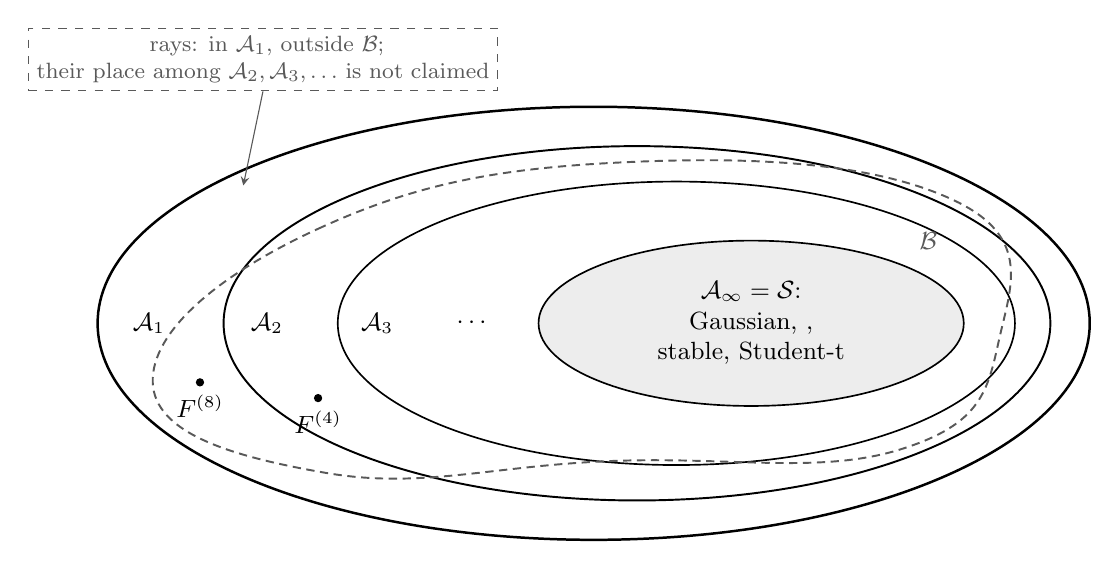
\begin{tikzpicture}[every node/.style={font=\small}, >=stealth]
% the chain
\draw[line width=0.9pt] (0,0) ellipse [x radius=6.3, y radius=2.75];
\draw[line width=0.7pt] (0.55,0) ellipse [x radius=5.25, y radius=2.25];
\draw[line width=0.6pt] (1.05,0) ellipse [x radius=4.3, y radius=1.8];
\draw[line width=0.6pt, fill=black!7] (2.0,0) ellipse [x radius=2.7, y radius=1.05];
\node at (-5.65,0) {$\mathcal{A}_1$};
\node at (-4.15,0) {$\mathcal{A}_2$};
\node at (-2.75,0) {$\mathcal{A}_3$};
\node at (-1.55,0) {$\cdots$};
\node[align=center] at (2.0,0) {$\mathcal{A}_\infty = \mathcal{S}$:\\ Gaussian, \Matern{},\\ stable, Student-t};
% the Bernstein class, a dashed contour
\draw[line width=0.7pt, densely dashed, gray!70!black]
  plot[smooth cycle, tension=0.75] coordinates
  {(-5.6,-0.75) (-3.5,1.2) (0.5,2.05) (4.6,1.55) (5.15,-0.2) (3.9,-1.6) (0.2,-1.75) (-3.4,-1.9)};
\node[gray!70!black] at (4.25,1.05) {$\mathcal{B}$};
% witnesses
\fill (-5.0,-0.75) circle (1.5pt) node[below=1pt] {$F^{(8)}$};
\fill (-3.5,-0.95) circle (1.5pt) node[below=1pt] {$F^{(4)}$};
% the Cin rays: outside B, position among the A_d not claimed
\node[draw, dashed, gray!70!black, align=center, font=\footnotesize, inner sep=3pt] (cin) at (-4.2,3.35)
  {$\Cin$ rays: in $\mathcal{A}_1$, outside $\mathcal{B}$;\\ their place among $\mathcal{A}_2, \mathcal{A}_3, \dots$ is not claimed};
\draw[->, gray!70!black] (cin.south) -- (-4.45,1.75);
\end{tikzpicture}
\caption{The dimension filtration, schematically. The class $\mathcal{A}_d$ holds the
admissible $F$ whose radial extension $F(|\xi|)$ is the exponent of a self-decomposable law on
$\RR^d$. The classes are nested, $\mathcal{A}_1$ is the whole admissible cone, and their
intersection is the image $\mathcal{S}$ of the bridge, which holds the named families, the
Student-t family under the hypothesis of Remark~\ref{rem:student-ggc}
(Proposition~\ref{prop:dimension-filtration}). The members $F^{(8)}$ and $F^{(4)}$ of
Lemma~\ref{lem:filtration-strictness} show that the first two inclusions are strict, and both
lie in the class $\mathcal{B}$ of the Bernstein condition, which contains
$\mathcal{A}_\infty$. Nothing is claimed about $\mathcal{B}$ against $\mathcal{A}_d$ for finite
$d > 1$, so $\mathcal{B}$ is a dashed contour and not a region of the chain. The $\Cin$ rays
lie outside $\mathcal{B}$, and the figure places them no more precisely than that.}
\label{fig:filtration}
\end{figure}
